\documentclass[a4paper,11pt]{article}

% Identificação
\newcommand{\pbtitulo}{Sqoop}
\newcommand{\pbversao}{1.00}

\usepackage{../sty/tutorial}

%----------------------------------------------------------------------
% Início do Documento
%----------------------------------------------------------------------
\begin{document}
	
	\maketitle % mostrar o título
	\thispagestyle{fancy} % habilitar o cabeçalho/rodapé das páginas
	
%--------------------------------------------------------------------------
% RESUMO DO ARTIGO
%--------------------------------------------------------------------------
\begin{abstract}
	% O primeiro caractere deve vir com \initial{}
	\initial{S}qoop\cite{sqoopoficial} ou "Apache Sqoop" e em 2021 foi movido para página da Attic para manutenções posteriores (aqui chamarei apenas de Sqoop) é parte do Ecosistema Hadoop criado para a criação e manutenção de software relacionado a \textit{Bulk Data Transfer} para Apache Hadoop e Datastores Estruturados.
\end{abstract}

%--------------------------------------------------------------------------
% CONTEÚDO DO ARTIGO
%--------------------------------------------------------------------------
\section{Parte inicial}
Sqoop é uma das ferramenta do ecossistema Hadoop usada para carregar dados de sistemas de gerenciamento de banco de dados relacional (RDBMS) para o Hadoop destinado ao processamento \textit{MapReduce} e exportá-los de volta ao RDBMS. Simplificando, o Sqoop auxilia no trafego para grandes quantidades de dados entrando e saindo do Hadoop com os bancos tradicionais.
\begin{figure}[H]
	\centering
	
\includegraphics[width=0.6\textwidth]{imagem/logo}
	\caption{Logo do Apache Sqoop}
\end{figure}

Sqoop nasceu da necessidade de muitos dos dados precisavam ser transferidos a partir de banco de dados relacionais para o Hadoop, havia a necessidade de uma ferramenta dedicada para fazer essa tarefa rapidamente. Foi aí que entrou em cena, amplamente usado para transferir esses dados.

Quando se trata de transferir dados, há um certo conjunto de requisitos a serem atendidos. Inclui o seguinte: \vspace{-1em}
\begin{itemize}
	\item Dados devem ter consistência.
	\item O aprovisionamento do pipeline de downstream. 
	\item Os usuários devem garantir o consumo dos recursos do sistema de produção
\end{itemize}
Lembremos que o \textit{MapReduce} não pode acessar diretamente os dados que residem em bancos de dados relacionais externos, deve buscá-los no \textit{Hadoop Distributed File System} (HDFS). Esse método pode expor o sistema ao risco como a geração de carga excessiva dos nós do cluster.

\begin{figure}[H]
	\centering
	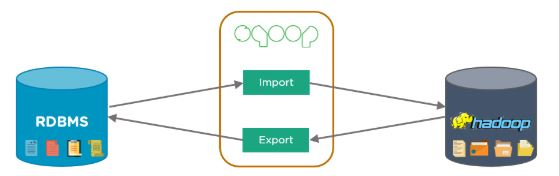
\includegraphics[width=0.8\textwidth]{imagem/transferencia.jpg}
	\caption{Funcionalidade do Sqoop}
\end{figure}

Para processar dados com o Hadoop é necessário que os dados precisam ser carregados em clusters do Hadoop de várias fontes. No entanto, descobriu-se que o processo para o carregamento dos dados de várias fontes heterogêneas era extremamente desafiador. Os problemas comuns que os administradores encontraram: \vspace{-1em}
\begin{itemize}
	\item Manter a consistência dos dados.
	\item Garantir a utilização eficiente dos recursos.
	\item Não era possível obter os dados em massa para o Hadoop.
	\item Carregar os dados ao utilizar \textit{script} era lento.
\end{itemize}

A solução foi Sqoop. O uso do Sqoop no Hadoop ajudou a superar todos os desafios da abordagem tradicional e pode carregar dados em massa do RDBMS para o Hadoop com facilidade. Devemos imaginar o fluxo de dados de uma empresa que executa uma importação noturna do Sqoop para carregar os dados do dia de um RDBMS transacional de produção em um \textit{data warehouse} do \textbf{Hive} para análise posterior. 

\section{Hadoop no Docker}
O modo mais simples de se conseguir trabalhar com o Hadoop é utilizando o Docker, para baixar a imagem do Hadoop: \\
\codigo{\$ docker pull suhothayan/hadoop-spark-pig-hive:2.9.2}

Nessa imagem temos outros produtos do Ecossistema Hadoop: Spark, Pig e Hive. Para criar e executar a primeira vez o contêiner (a pasta que este comando for executado será associada a uma pasta interna chamada \textbf{/home/tsthadoop}): \\
\codigo{\$ docker run -it -d --name meu-hadoop -v \$(pwd):/home/tsthadoop \\ suhothayan/hadoop-spark-pig-hive:2.9.2}

Uma vez interrompido o contêiner: \\
\codigo{\$ docker stop meu-hadoop}

Podemos executá-lo novamente com os seguintes comandos: \\
\codigo{\$ docker start meu-hadoop \\
\$ docker exec -it meu-hadoop /etc/bootstrap.sh bash}

\subsection{Erro de Permissão}
Na primeira vez que entramos é dado um erro na execução do script "bootstrap.sh" de permissão negada para executar o script "spark-env.sh", vamos corrigir isso com o comando: \\
\codigo{\# chmod 777 /usr/local/spark/conf/spark-env.sh}

Vamos sair do bash: \\
\codigo{\# exit}

Podemos executá-lo novamente: \\
\codigo{\$ docker exec -it meu-hadoop /etc/bootstrap.sh bash}

E o erro desapareceu.


\subsection{Instalar o Sqoop}
Porém se leu corretamente essa imagem NÃO POSSUI o Sqoop e agora realmente começa nossa instalação, optei por utilizar essa imagem por já possuir todos os componentes necessários para posterior tratamento dos dados. Desta forma ao invés de realizar um trabalho de obter uma imagem somente com o Sqoop (que existem várias por aí e ter que instalar todos os outros componentes), vamos utilizar uma imagem que estamos acostumados e que já possui todas as outras ferramentas necessárias e nos preocuparmos apenas com o Sqoop.

Outros ganho adicionais desse método é que também pode ser excelente para aprendermos como se adiciona uma ferramenta ao ecossistema do Hadoop além de não ficarmos presos a uma determinada versão (que muitas imagens ainda estão com a versão 1.4.7). E agora podemos "brincar" melhor com as outras ferramentas como o Spark, Hive e Pig que já estão nessa imagem.

No endereço oficial \cite{scoopoficial} existe o link para Download, acessando este vemos todas as versões disponíveis, utilizaremos a última até o momento, clicar no link "1.99.7" e baixar o arquivo \textbf{sqoop-1.99.7-bin-hadoop200.tar.gz} e colocá-lo na pasta associativa da imagem.

Retornar a pasta raiz do root: \\
\codigo{\# cd root/}

Descompactar o arquivo: \\
\codigo{\# tar vfx /home/tsthadoop/sqoop-1.99.7-bin-hadoop200.tar.gz}

Mover o pasta descompactada para o endereço local (aonde estão os outros produtos do Ecossistema): \\
\codigo{\# mv sqoop-1.99.7-bin-hadoop200 /usr/local/.}

Criar um link simbólico para facilitar o acesso: \\
\codigo{\# ln -s /usr/local/sqoop-1.99.7-bin-hadoop200 sqoop}

No arquivo core-site.xml do Hadoop habilitar os acessos, editar o arquivo: \\
\codigo{\# vim \$HADOOP\_PREFIX/etc/hadoop/core-site.xml.template}

Pressionar "i" para entrar em modo de edição e adicionar as seguintes propriedades:
\begin{lstlisting}[]
<property>
  <name>hadoop.proxyuser.sqoop2.hosts</name>
  <value>*</value>
</property>
<property>
  <name>hadoop.proxyuser.sqoop2.groups</name>
  <value>*</value>
</property>
\end{lstlisting}

Pressionar "ESC" para sair do modo de edição e salvar o arquivo pressionando ":wq". Na pasta de configuração do Sqoop precisamos modificar o caminho do Hadoop, editar o arquivo: \\
\codigo{\# vim /usr/local/sqoop/conf/sqoop.properties}

Localizar a linha: \\
\codigo{\# Hadoop configuration directory}

E modificar o valor da variável (entrar em modo de edição pressionando a tecla "i") para:
\begin{lstlisting}[]
org.apache.sqoop.submission.engine.mapreduce.configuration.directory = /usr/local/hadoop/share/hadoop/mapreduce
\end{lstlisting}

Pressionar "ESC" para sair do modo de edição e salvar o arquivo pressionando ":wq". O Sqoop precisa acessar bancos de dados, sendo assim precisamos adicionar os arquivos JAR de JDBC dos bancos que desejamos inserir. Criar uma pasta: \\
\codigo{\# mkdir -p /var/lib/sqoop2/}

Copiar para esta pasta os arquivos JAR necessários. Vamos modificar o arquivo "etc/bootstrap.sh" o seguinte EXPORT: \\
\codigo{\# vim /etc/bootstrap.sh}

E adicionar as seguintes linhas abaixo dos comandos EXPORT:
\begin{lstlisting}[]
export PATH=$PATH:/usr/local/sqoop/bin
export SQOOP_SERVER_EXTRA_LIB=/var/lib/sqoop2/
\end{lstlisting}

Aproveitamos e inserimos o caminha do path para a pasta do Sqoop. Pressionar "ESC" para sair do modo de edição e salvar o arquivo pressionando ":wq".  Sair da imagem, parar e iniciar o contêiner, entrar no bash novamente.

Acessar a pasta associativa: \\
\codigo{\# cd /home/tsthadoop}

Verificar se o Sqoop está correto: \\
\codigo{\# sqoop2-tool verify}

Se aparecer a mensagem "\textit{Verification was successful.}" está tudo bem, porém caso mostrar "\textit{Verification has failed, please check Server logs for further details.}" devemos verificar o arquivo de Log que se encontra nas pasta @LOGDIR@.

\subsection{Executar o Sqoop}

Com tudo OK, executamos o servidor do Sqoop: \\
\codigo{\# sqoop2-server start}

Que deve mostrar a mensagem "\textit{Sqoop2 server started.}". Por padrão utiliza a porta 12000. Podemos modificar a porta na variável "org.apache.sqoop.jetty.port" no arquivo de configuração em "conf/sqoop.properties". Podemos pará-lo com o comando: \\
\codigo{\# sqoop2-server stop}

Acessar o cliente: \\
\codigo{\# sqoop2-shell}

Ver os comando disponíveis: \\
\codigo{sqoop:000> help}

Agora vamos a parte divertida, a real utilidade do Sqoop que é Importar/Exportar dados de RDBS, para isso utilizamos \textit{Java Database Connectivity} (JDBC).

\section{Passos Iniciais}
Acessar a pasta associativa: \\
\codigo{\# cd /home/tsthadoop}

Iniciar o servidor: \\
\codigo{\# sqoop2-server start}

Com a resposta: "\textit{Sqoop2 server started.}" acessar o cliente: \\
\codigo{\# sqoop2-shell}

Verificar a versão: \\
\codigo{sqoop:000> show version -a}

Conectar o cliente ao servidor: \\
\codigo{sqoop:000> set server --host 172.17.0.2 --port 12000 --webapp sqoop}

Após mostrar a mensagem "\textit{Server is set successfully}", verificar se fez efeito: \\
\codigo{sqoop:000> show server -a}

Ver os conectores disponíveis: \\
\codigo{sqoop:000> show connector}

Ao adicionar a opção -a teremos mais informação: \\
\codigo{sqoop:000> show connector -a}

Podemos usar essa opção -a para todos os comandos "show". Porém isso não afetara as respostas quando estivermos importando ou exportando dados, assim vamos deixar o Sqoop nos responder de modo verboso: \\
\codigo{sqoop:000> set option --name verbose --value true}

Verificar se fez efeito: \\
\codigo{sqoop:000> show option}

Sair do cliente: \\
\codigo{sqoop:000> :x}

Encerrar o servidor do Sqoop: \\
\codigo{\# sqoop2-server stop}

\section{Criar uma conexão}
Para realizar uma conexão com qualquer RDBMS precisamos de conectores registrados, um deles cria uma conexão JBDC e é esse que utilizaremos, porém precisamos ter o banco de dados a nossa disposição, já que estamos usando o Docker podemos sair do contêiner e criar um novo com o banco que desejamos testar, aqui utilizaremos o MySQL e que este sirva como ponto de partida e entendimento para qualquer outro pois a conexão é basicamente a mesma.

Baixar a imagem oficial: \\
\codigo{\$ docker pull mysql}

Criar uma instância do banco em um Contêiner: \\
\codigo{\$ docker run --name meu-mysql -e MYSQL\_ROOT\_PASSWORD=root -p 3306:3306 -d mysql}

Nas próximas vezes, usamos para iniciar o MySQL: \\
\codigo{\$ docker start meu-mysql}

Parar o MySQL: \\
\codigo{\$ docker stop meu-mysql}

Entrar diretamente no gerenciador o comando: \\
\codigo{\$ docker exec -it meu-mysql sh -c 'exec mysql -u root -p'}

Ou então: \\
\codigo{\$ docker exec -it meu-mysql bash \\
\# mysql -u root -p}

No MySQL precisamos de um banco, no gerenciado criamos: \\
\codigo{mysql> CREATE DATABASE tstsqoop;}

Entrar no banco criado:
\codigo{mysql> USE tstsqoop;}

Criamos as tabelas que realizaremos as importações e exportações de dados: \\
\codigo{mysql> CREATE TABLE recebimento (codigo int not null, estado char(2), \\ 
valorrec float(5,2), PRIMARY KEY (codigo)); \\
mysql> CREATE TABLE analitico (estado char(2), valortotal float(8,2), \\ 
PRIMARY KEY (estado));}

A tabela de recebimento contém os valores recebidos dos estados, esses devem ser contabilizados na tabela analítico. Adicionamos alguns registros na tabela recebimento: \\
\codigo{mysql> INSERT INTO recebimento VALUES (1, 'DF', 120.00); \\
mysql> INSERT INTO recebimento VALUES (2, 'DF', 180.00); \\
mysql> INSERT INTO recebimento VALUES (3, 'DF', 80.00); \\
mysql> INSERT INTO recebimento VALUES (4, 'MG', 132.30); \\
mysql> INSERT INTO recebimento VALUES (5, 'MG', 22.60);}

Adicionar outros pois quanto mais valores melhor. E nosso trabalho aqui está feito, sair do MySQL: \\
\codigo{mysql> quit}

NÃO parar este contêiner pois precisamos dele ativo. Agora necessitamos de um drive JDBC de conexão, este é um arquivo padrão \textbf{.JAR} que pode ser obtido gratuitamente em vários sites. Por exemplo em \url{https://downloads.mysql.com/archives/c-j/}, selecionar como sistema operacional "\textit{Platform Independent}". Descompactar o arquivo que foi realizado dowload e neste encontramos um arquivo .JAR chamado "mysql-connector-java-8.0.27.jar".

Copiar esse arquivo para o diretório compartilhado na máquina local, vamos retornar para o contêiner do Hadoop: \\
\codigo{\$ docker exec -it meu-hadoop2 /etc/bootstrap.sh bash}

Acessar a pasta das bibliotecas JDBC do Sqoop: \\
\codigo{\# cd /var/lib/sqoop2/}

Copiar o arquivo JDBC: \\
\codigo{\# mv /home/tsthadoop/mysql-connector-java-8.0.27.jar .}

Acessar a pasta associativa: \\
\codigo{\# cd /home/tsthadoop}

Copiar os dois arquivos conectores que realizam a conexão nesta pasta: \\
\codigo{\# cp /usr/local/sqoop-1.99.7-bin-hadoop200/server/lib/ \\ sqoop-connector-generic-jdbc-1.99.7.jar . \\
\# cp /usr/local/sqoop-1.99.7-bin-hadoop200/server/lib/ \\
sqoop-connector-hdfs-1.99.7.jar .}

Iniciar o servidor: \\
\codigo{\# sqoop2-server start}

Com a resposta: "\textit{Sqoop2 server started.}" acessar o cliente: \\
\codigo{\# sqoop2-shell}

Verificar se o servidor está conectado: \\
\codigo{sqoop:000> show server -a}

Caso não esteja conectar o cliente ao servidor. Criar um link de conexão com o banco: \\
\codigo{sqoop:000> create link -connector generic-jdbc-connector}

Os parâmetros são:
\begin{lstlisting}[]
Name: Link com MySQL
Driver Class: com.mysql.cj.jdbc.Driver
JDBC Connection String: jdbc:mysql://[IP da Máquina]/tstsqoop
Username: root
Password: root
Fetch Size:
entry# protocol = tcp
entry# useSSL = false
entry# 
Identifier enclose: [colocar um espaço aqui]
\end{lstlisting}

Ao término mostra que foi estabelecido uma Conexão com o banco MySQL. A beleza é que ao criar um contêiner do MySQL é como se esse tivesse instalado na nossa máquina local pois existe uma associação com a porta 3606, por isso informamos o IP da Máquina local ao invés do IP do Contêiner. Os parâmetros que estão em brancos basta pressionar a tecla ENTER.

O parâmetro \textit{Identifier enclose} deve ser colocado um espaço, pois caso contrário tentará colocar $"$ (aspas duplas) na chamada do schema (que não existe para o conector do MySQL) e na tabela.

Criar um link com o HDFS do Hadoop, com o comando: \\
\codigo{sqoop:000> create link -connector hdfs-connector}

Os parâmetros são:
\begin{lstlisting}[]
Name: Link com Hadoop
URI: hdfs://localhost:9000
Conf directory: /usr/local/hadoop/etc/hadoop
entry#
\end{lstlisting}

Verificar os links criados: \\
\codigo{sqoop:000> show link}

Mudar qualquer opção utilizar o comando: \\
\codigo{sqoop:000> update link -name $"$[nome link]$"$}

Eliminar um link:
\codigo{sqoop:000> delete link -name $"$[nome link]$"$}

\section{Importar Dados}
Este é o processo no qual as tabelas individuais são importadas do RDBMS para o HDFS. Para fins de transferência, a linha em uma tabela é considerada um registro no HDFS. Os dados gravados são armazenados na forma de dados de texto em arquivos de texto ou são armazenados em arquivos Sequence e Avro como dados binários.

Importação (ou mesmo a Exportação) de dados é o movimento de um link para outro, isso é realizado através de um Job, para criarmos o Job de Importação usamos: \\
\codigo{sqoop:000> create job -f $"$Link com MySQL$"$ -t $"$Link com Hadoop$"$ }

Os parâmetros são:
\begin{lstlisting}[]
Name: Recebimento
Schema name:
Table name: recebimento
SQL statement:
Column names:
element# estado
element# valorrec
element#
Partition column: codigo
Partition column nullable:
Boundary query:
Check column:
Last value:
Override null value:
Null value:
File format: 0
Compression codec: 0
Custom codec:
Output directory: hdfs://localhost:9000/user/root/tstsqoop
Append mode:
Extractors: 1
Loaders: 1
Extra mapper jars:
There are currently 0 values in the list:
element#
\end{lstlisting}

Como resposta temos: \textit{New job was successfully created with validation status OK and name Recebimento}. Podemos ver o Job com: \\
\codigo{sqoop:000> show job}

Para executar o Job: \\
\codigo{sqoop:000> start job -name Recebimento}

Os dados foram colocados no HDFS e aplicado um Map/Reduce, saímos do shell do Sqoop: \\
\codigo{sqoop:000> :x}

Verificamos a pasta destino do HDFS: \\
\codigo{\# hdfs dfs -ls /user/root/tstsqoop}

E encontraremos o arquivo (ATENÇÃO os números podem variar pois são gerados automaticamente com base em um HASH) importado, no MEU caso o arquivo é:
\begin{lstlisting}[]
Found 1 items
-rw-r--r--   1 root supergroup         20 2022-04-03 17:42 /user/root/tstsqoop/60ce7fbc-1d59-4da1-ae2a-86591beae4d8.txt
\end{lstlisting}

Verificamos seu conteúdo com: \\
\codigo{\# hdfs dfs -cat /user/root/tstsqoop/60ce7fbc-1d59-4da1-ae2a-86591beae4d8.txt}

E veremos os dados do banco MySQL conforme solicitado. Que podemos utilizar para realizar um Map/Reduce ou qualquer outra ação.

Mais fontes de informação podem ser obtidas em diversos sites que apresenta tutoriais completos sobre o Sqoop como a Tutorials Point\cite{tutorialspoint}.

\section{Conclusão}
É inegável que para quem utiliza Hadoop, o trabalho interessante começa depois que os dados são carregados no HDFS. Os desenvolvedores podem "brincar" com os dados para encontrar os \textit{insights} mágicos ocultos nesse Big Data. Para isso, os dados que residem nos sistemas de RDBS precisam ser transferidos ao HDFS, trabalhar com os dados e serem enviados de volta aos RDBS. A realidade do mundo \textbf{Big Data}, os desenvolvedores sentem que a transferência de dados entre sistemas RDBS e HDFS não é tão interessante, tediosa, mas necessária. Os desenvolvedores sempre podem escrever scripts personalizados para transferir dados para dentro e para fora do Hadoop (que como já visto é um processo mais lento), assim o Sqoop oferece uma alternativa excelente para resolver esse problema.

Sqoop automatiza a maior parte do processo, depende do banco de dados para descrever o esquema dos dados a serem importados. Utiliza a estrutura MapReduce para importar e exportar os dados, que fornece mecanismo paralelo e tolerância a falhas. Facilita a vida dos administradores ao fornecer uma interface de linha de comando. Necessitamos apenas inserir informações básicas como detalhes de autenticação de origem, destino e banco de dados no comando Sqoop que cuida da parte restante. 

Sou um entusiasta do mundo \textbf{Open Source} e novas tecnologias. Qual a diferença entre Livre e Open Source? \underline{Livre} significa que esta apostila é gratuita e pode ser compartilhada a vontade. \underline{Open Source} além de livre todos os arquivos que permitem a geração desta (chamados de arquivos fontes) devem ser disponibilizados para que qualquer pessoa possa modificar ao seu prazer, gerar novas, complementar ou fazer o que quiser. Os fontes da apostila (que foi produzida com o LaTex) está disponibilizado no GitHub \cite{github}. Veja ainda outros artigos que publico sobre tecnologia através do meu Blog Oficial \cite{fernandoanselmo}.

%--------------------------------------------------------------------------
% REFERÊNCIAS
%--------------------------------------------------------------------------
\begin{thebibliography}{4}
	\bibitem{sqoopoficial} 
	Página do Sqoop \\
	\url{https://attic.apache.org/projects/sqoop.html}

	\bibitem{tutorialspoint} 
	Tutorials Point sobre Sqoop \\
	\url{https://www.tutorialspoint.com/sqoop/index.htm}
	
		\bibitem{fernandoanselmo} 
	Fernando Anselmo - Blog Oficial de Tecnologia \\
	\url{http://www.fernandoanselmo.blogspot.com.br/}
	
	\bibitem{publicacao} 
	Encontre essa e outras publicações em \\
	\url{https://cetrex.academia.edu/FernandoAnselmo}
	
	\bibitem{github} 
	Repositório para os fontes da apostila \\
	\url{https://github.com/fernandoans/publicacoes}
\end{thebibliography}

\end{document}